\documentclass[12pt]{article}

\usepackage{graphicx}
\usepackage{listings}
\usepackage{hyperref}
\usepackage{float}

\graphicspath{ {./images/} }

\oddsidemargin 0mm
\evensidemargin 0mm
\textwidth 160mm
\textheight 200mm

\pagestyle {plain}
\pagenumbering{arabic}

\newcounter{stepnum}

\title{CS/SE 2XC3 Lab 2 Report}
\author{
  Glotov, Oleg\\ L03, 400174037\\
  \texttt{glotovo@mcmaster.ca}
  \and
  Willson, Emma\\ L02, 400309856\\
  \texttt{willsone@mcmaster.ca}
  }
\date{\today}

\begin{document}

\maketitle

This report includes the main observations that we found in this week's lab, along with the analysis of our results.

\newpage 
\section{Timing Data}
In this section, we analyze the test results of three functions and give our best judgement of how each of these functions is growing in $n$.
\subsection{\(f(n)\)}
For the data set of $f(n)$, the trend line appears to be linear. From the chart below we can see that the $R^2$ is 0.9992 for the linear equation. It is already a very good result.

\begin{figure}[h!]
\centering
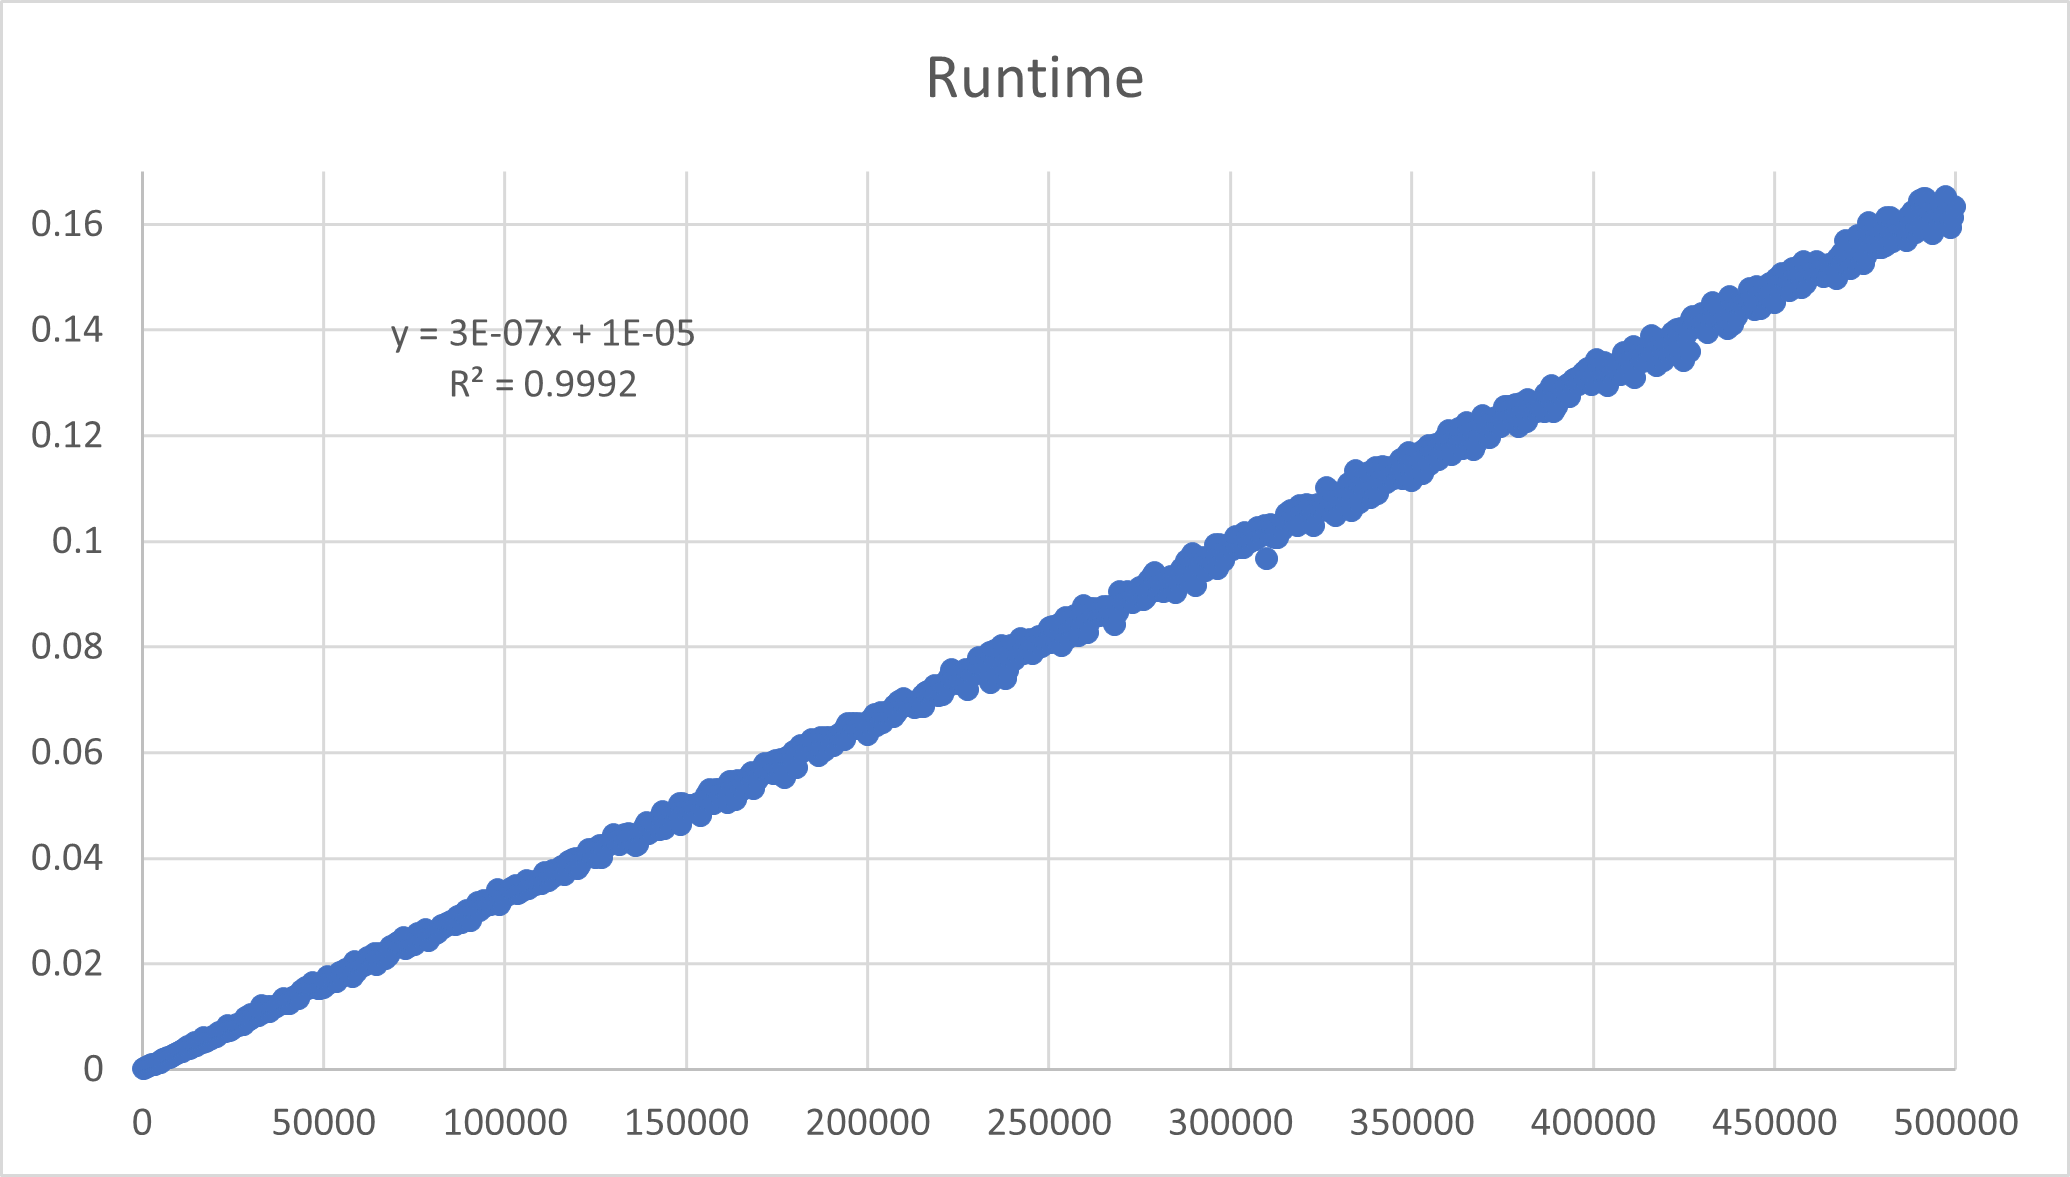
\includegraphics[width=0.6\textwidth,height=\textheight,keepaspectratio]{fn_Tn}
\caption{linear fitting for $f(n)$}
\label{Figure: fn_1}
\end{figure}
\noindent Therefore, we can conclude that $f(n) = O(n)$. 

\subsection{\(g(n)\)}
When we graph the data set for $g(n)$, the trend line appears to be polynomial. From the chart below we can see that the $R^2$ is 0.9883 for the quadratic equation. 

\begin{figure}[H]
\centering
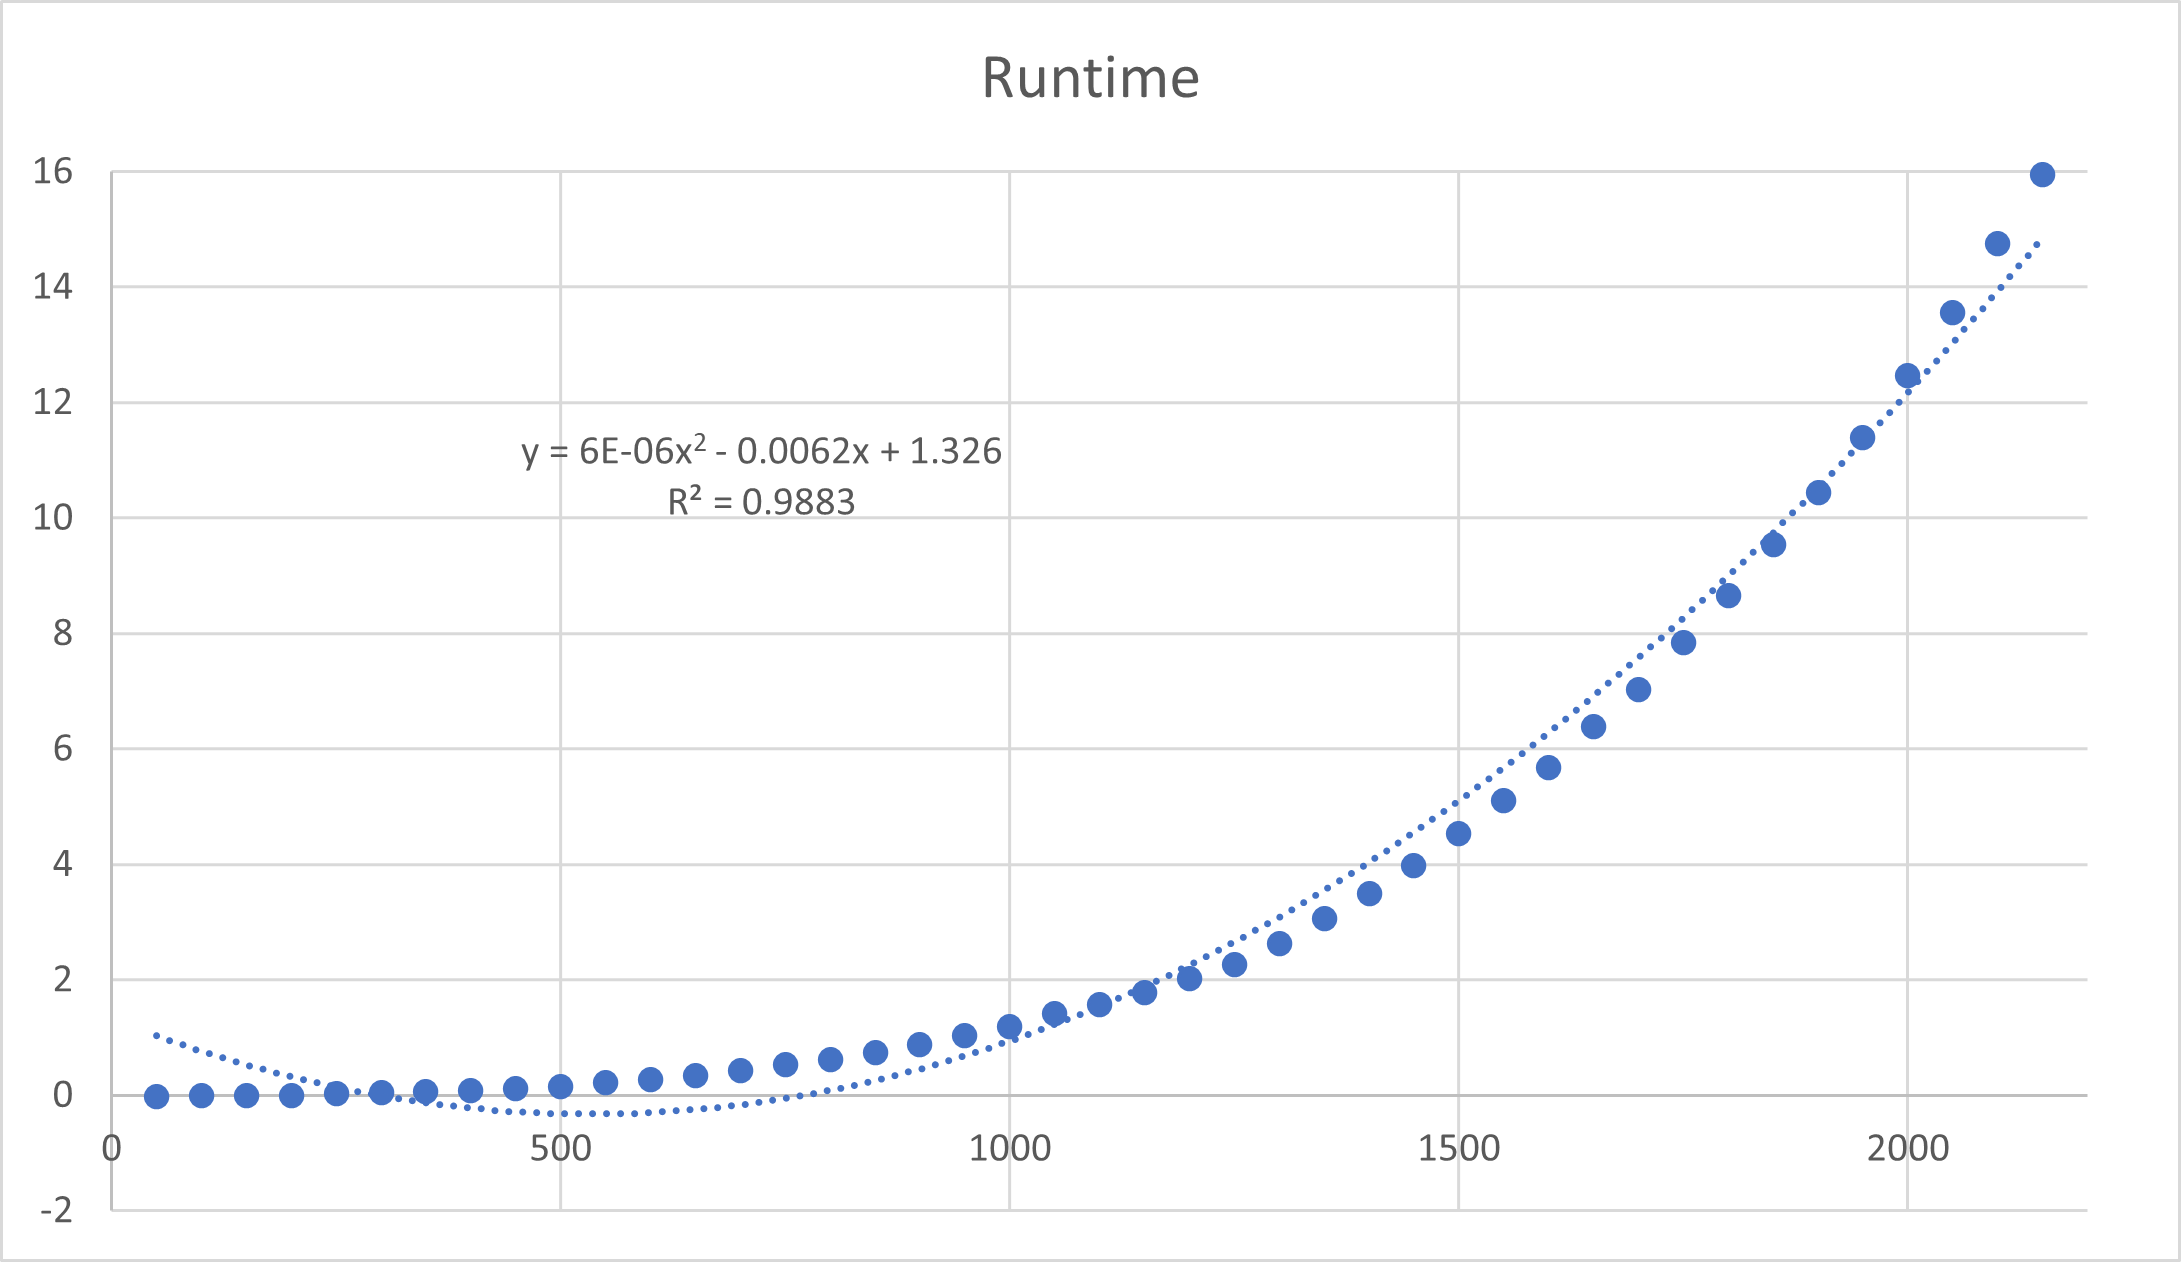
\includegraphics[width=0.6\textwidth,height=\textheight,keepaspectratio]{gn_Tn}
\caption{polynomial fitting for $g(n)$}
\label{Figure: gn_1}
\end{figure}

\noindent We will try to improve the $R^2$ by finding the value of $k$ in $T(n) = cn^k$. We do so by taking the logarithm of both sides of this equation: $\log{T}=\log{c}+k\log{n}$ and plotting $\log{T}$ against $\log{n}$. 

\begin{figure}[H]
\centering
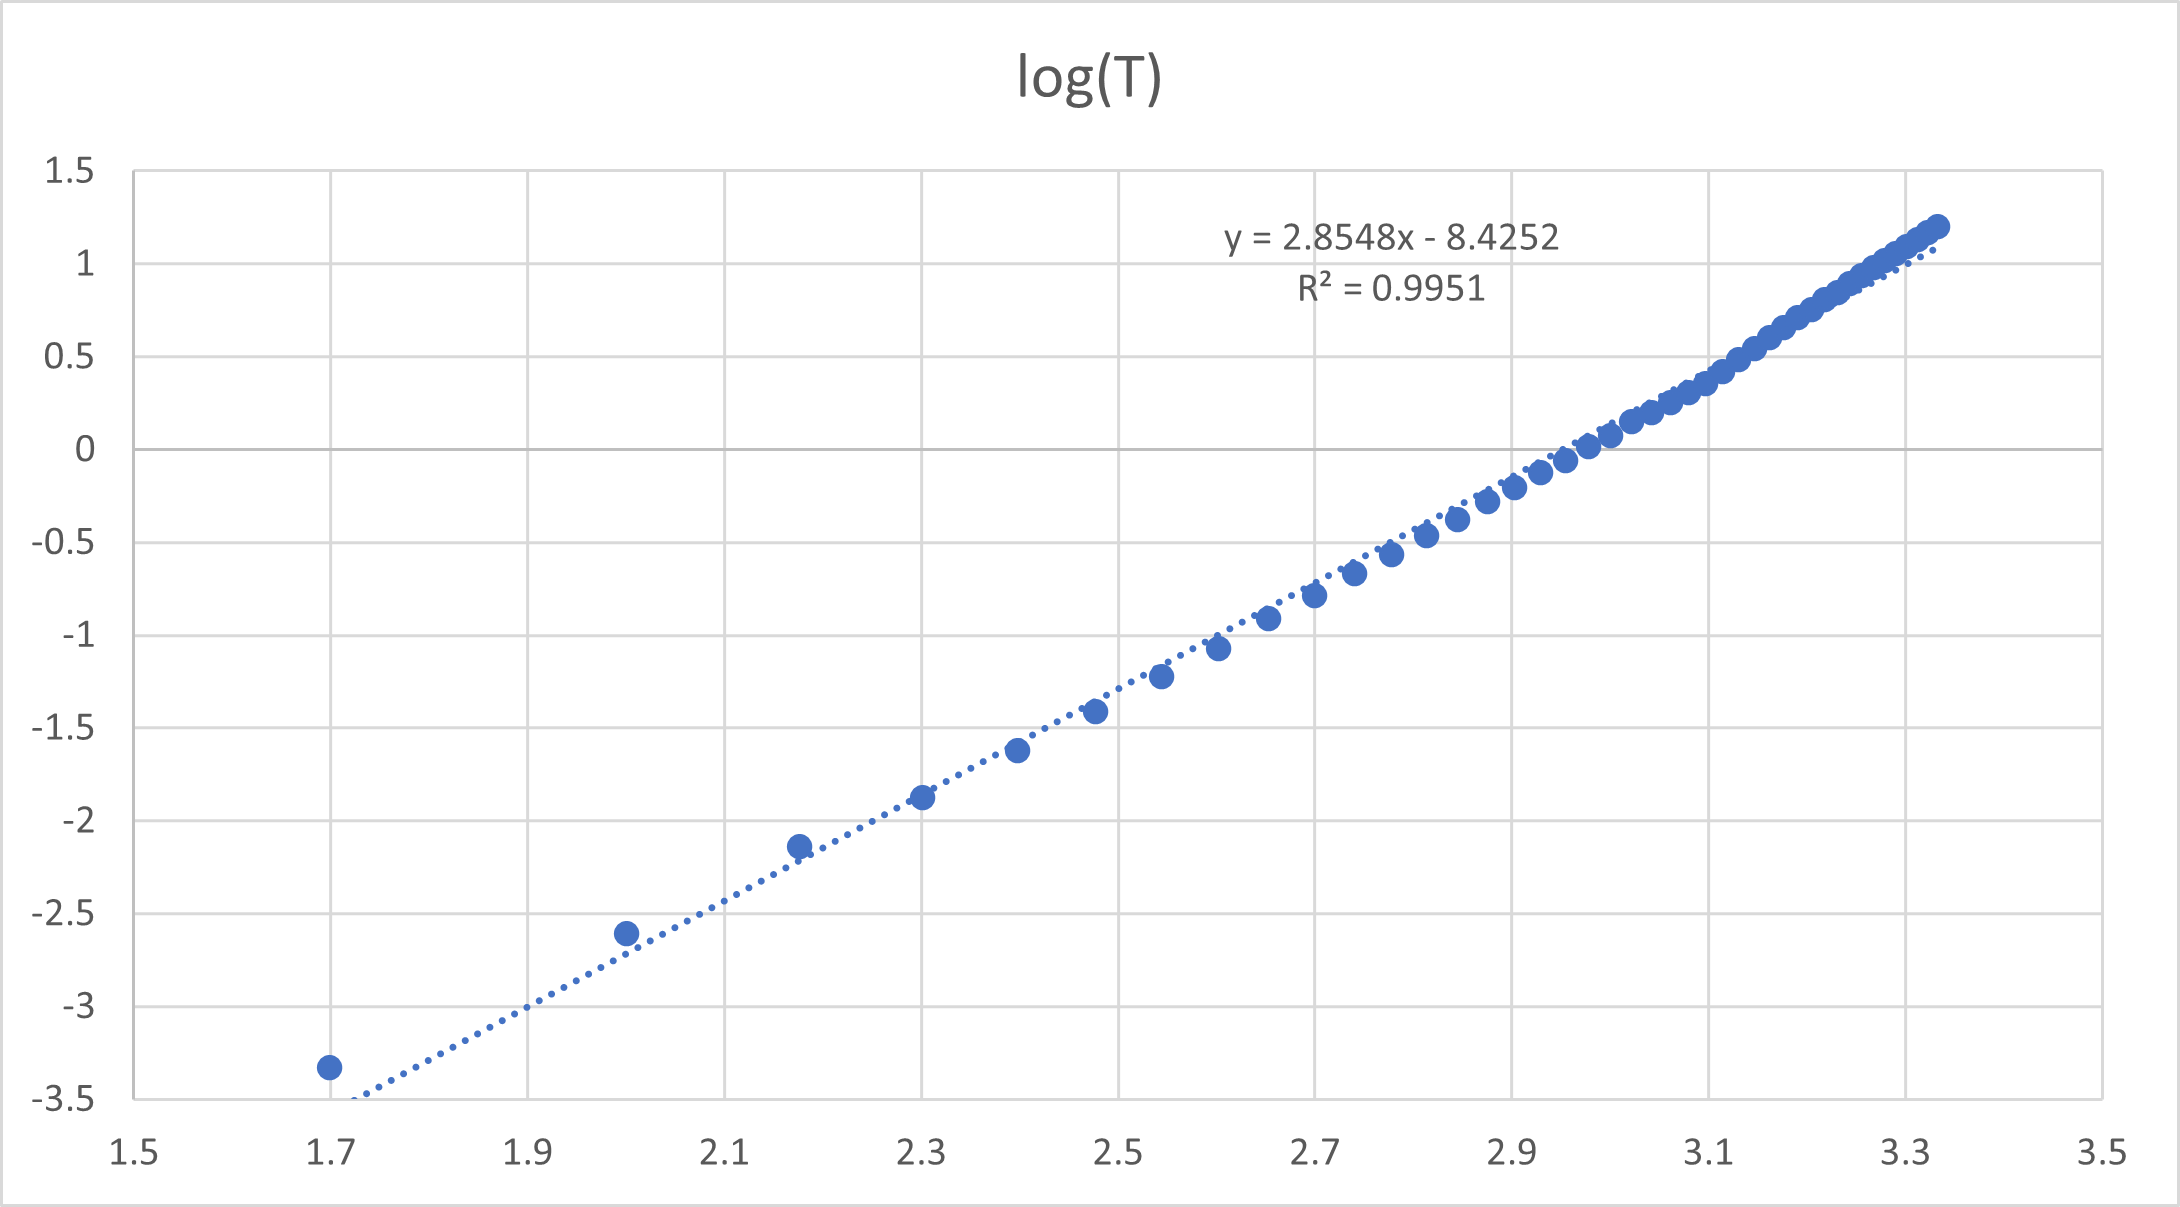
\includegraphics[width=0.6\textwidth,height=\textheight,keepaspectratio]{gn_logT}
\caption{polynomial fitting for $\log{T}$}
\label{Figure: gn_2}
\end{figure}

\noindent When we choose a linear trend line for this relation, we see that $k$, the slope, is 2.8548, which is closer to 3. When we recalculate the polynomial trend line for the original data with $k=3$, we see that this is a better fit.

\begin{figure}[H]
\centering
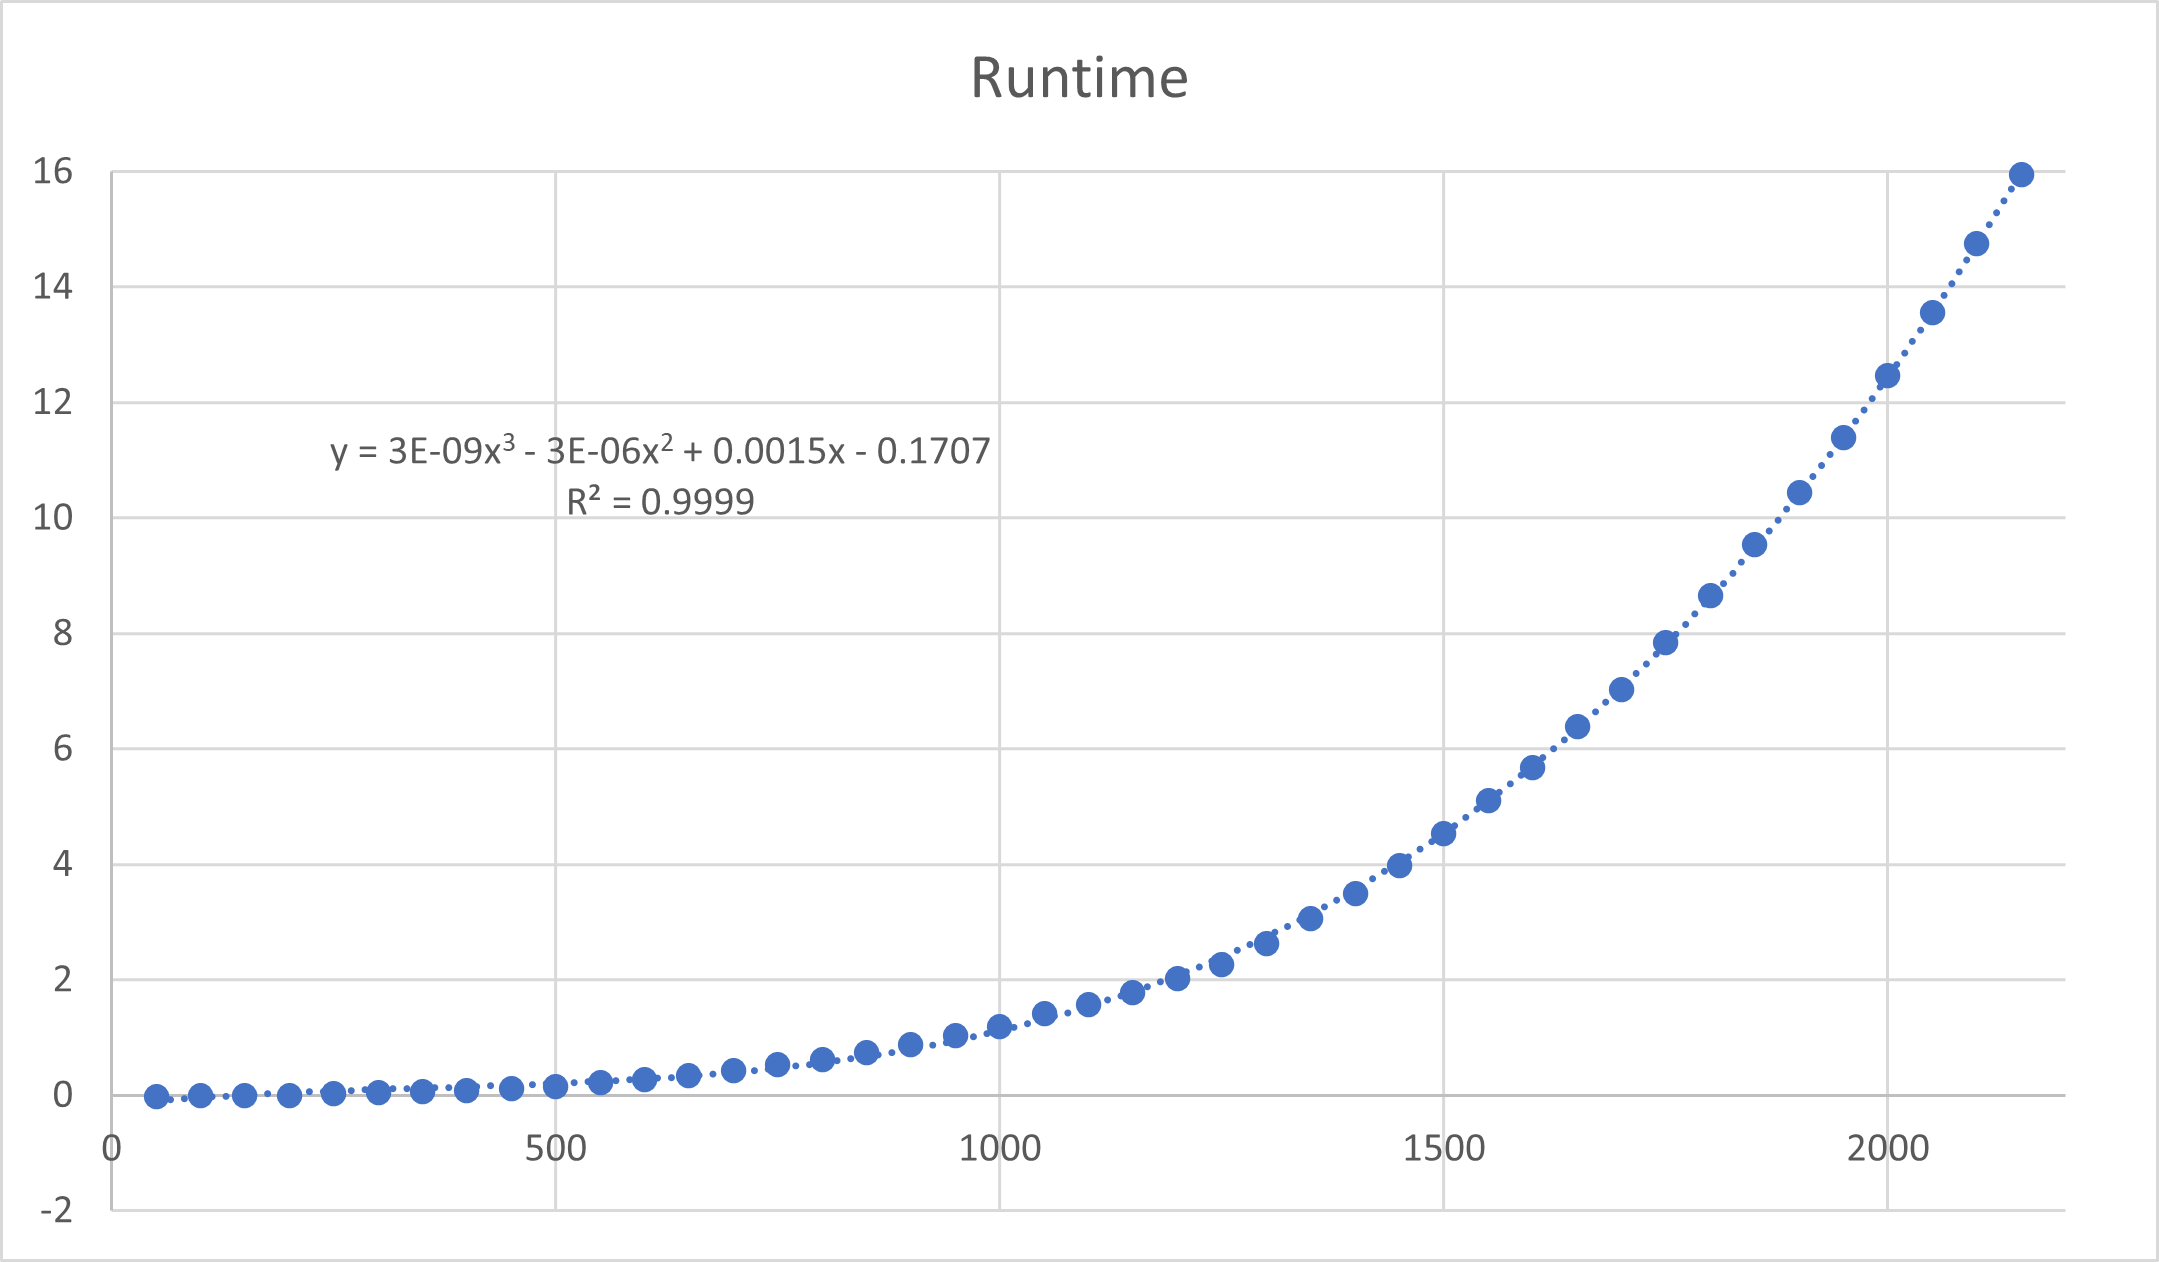
\includegraphics[width=0.6\textwidth,height=\textheight,keepaspectratio]{gn_Tn2}
\caption{linear fitting for $g(n)$}
\label{Figure: gn_3}
\end{figure}

\noindent Here, the $R^2$ is 0.9999, which is a very good result. Therefore we can conclude that $g(n) = O(n^3)$.

\subsection{\(h(n)\)}
When we graph the data set for $h(n)$, the trend line appears to be linear. From the chart below we can see that the $R^2$ is 0.9976 for the linear equation. This is already pretty good, but we might be able to improve it.

\begin{figure}[H]
\centering
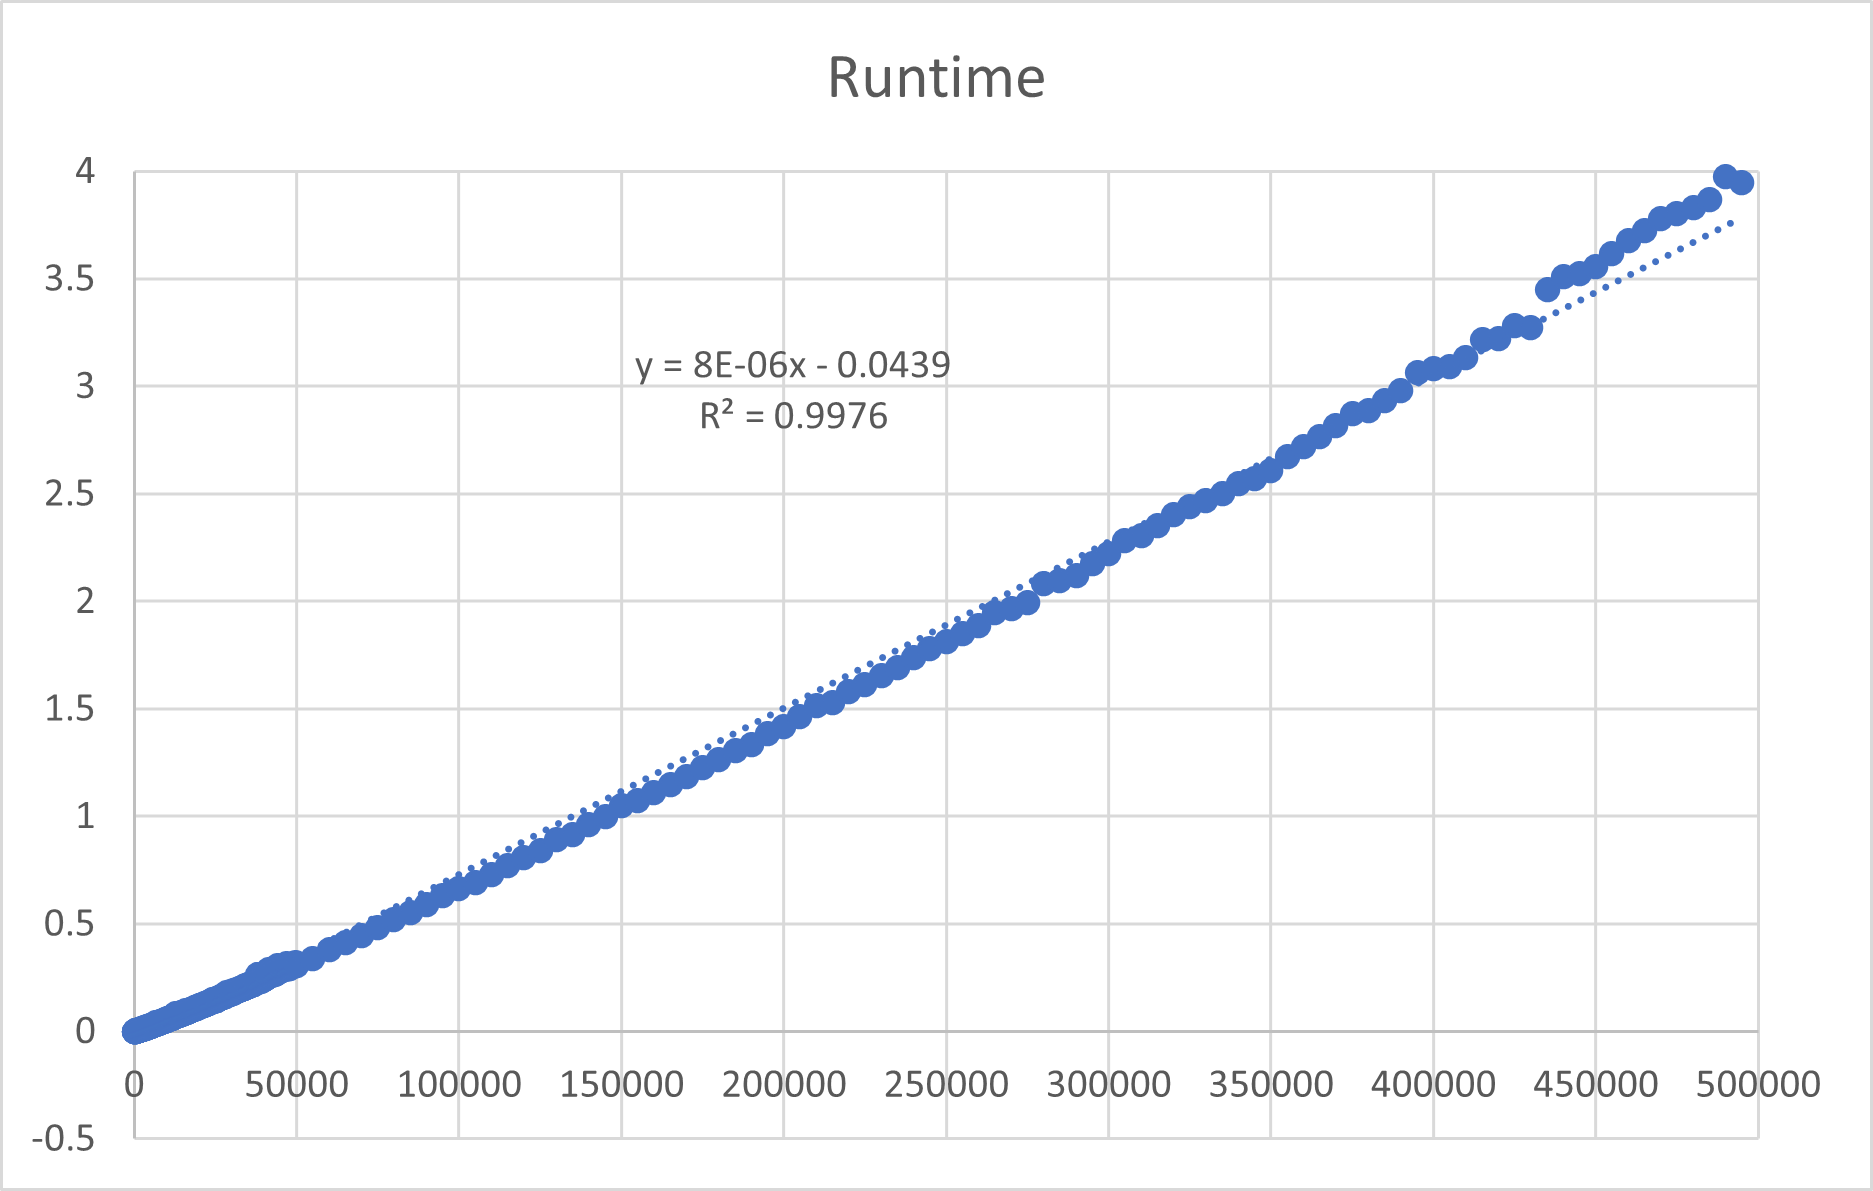
\includegraphics[width=0.6\textwidth,height=\textheight,keepaspectratio]{hn_Tn}
\caption{linear fitting for $h(n)$}
\label{Figure: hn_1}
\end{figure}

\noindent First, we will check the value of $k$ in $T(n) = cn^k$. We do so by taking the logarithm of both sides of this equation: $\log{T}=\log{c}+k\log{n}$ and plotting $\log{T}$ against $\log{n}$. 

\begin{figure}[H]
\centering
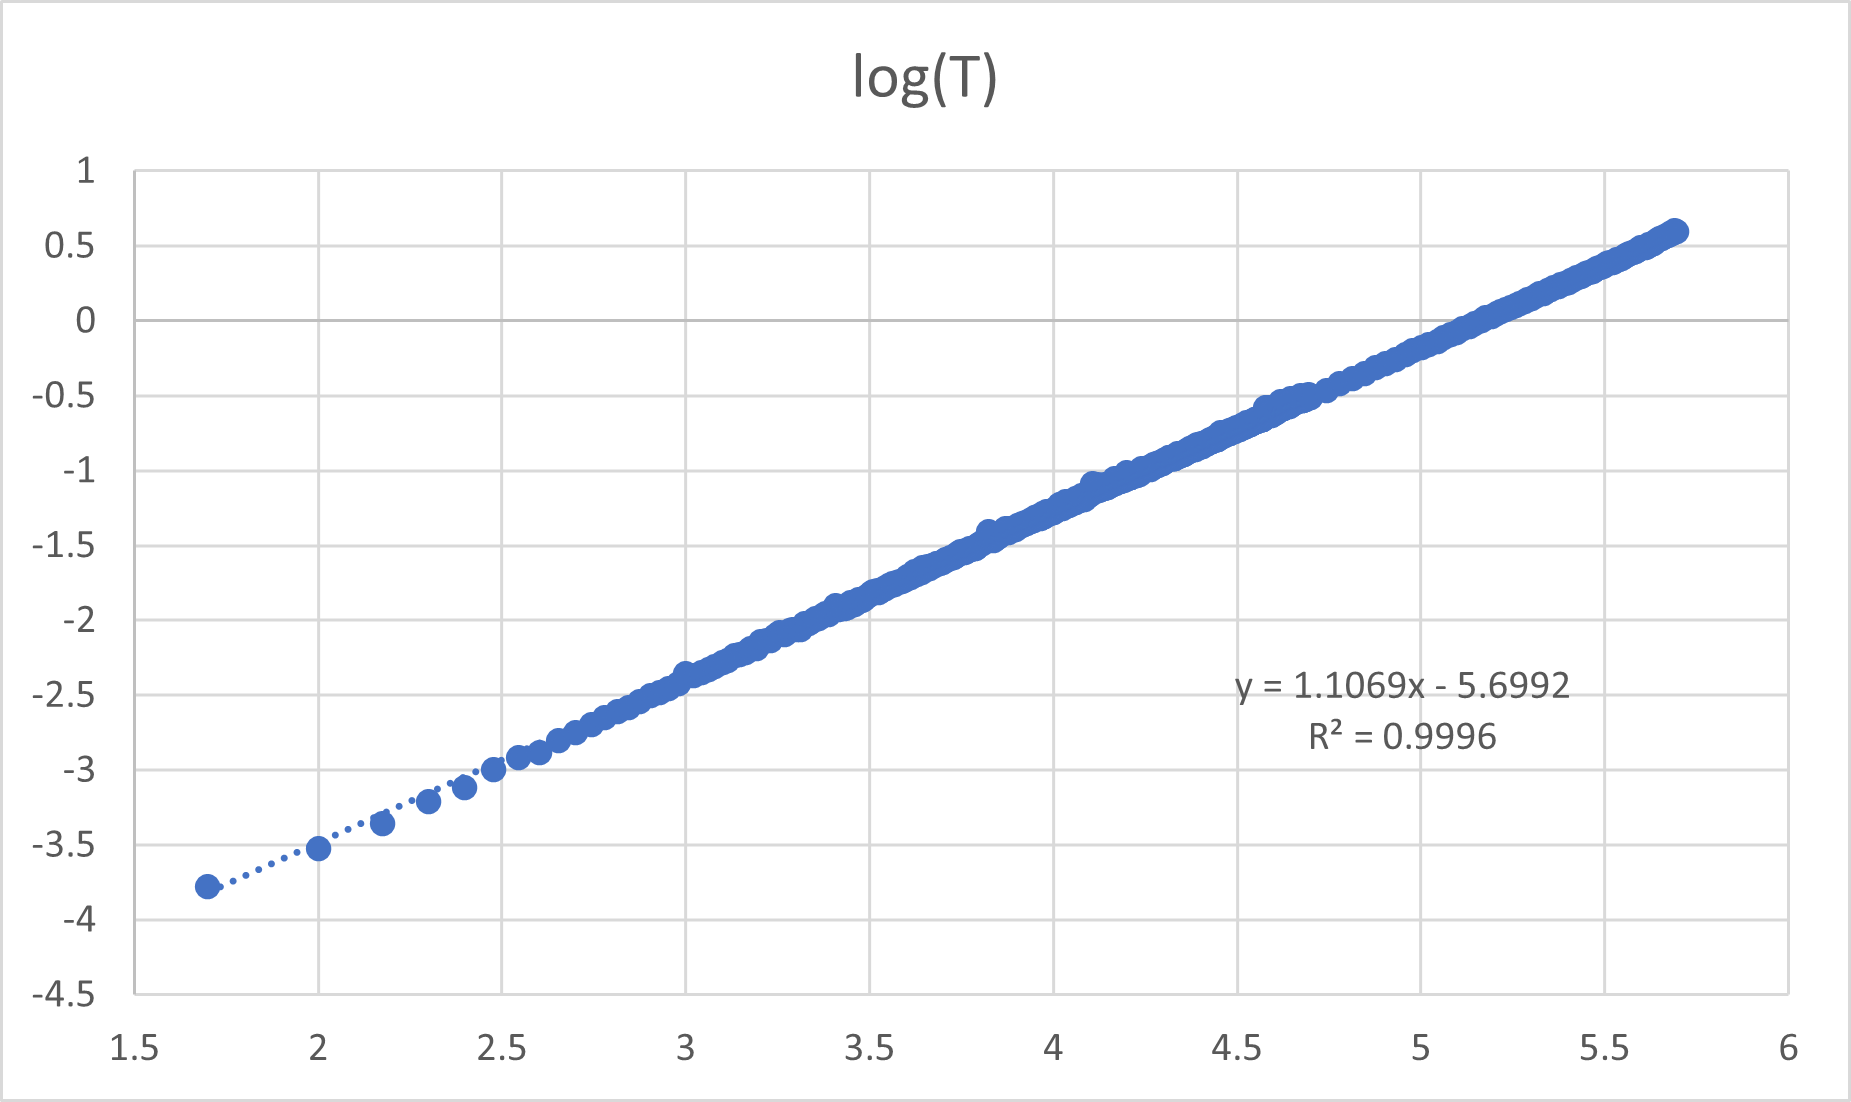
\includegraphics[width=0.6\textwidth,height=\textheight,keepaspectratio]{hn_logT}
\caption{linear fitting for $\log{T}$}
\label{Figure: hn_2}
\end{figure}

\noindent When we choose a linear trend line for this relation, we see that $k$, the slope, is 1.1069. Since $k$ represents the exponent on $n$ in the original data set, this makes the time complexity almost linear. However, $O(n\log{n})$ may be a better fit than $O(n)$. We can check which is better by plotting $\frac{T(n)}{n}$ against $n$. If $T(n) = cn$, then the resulting graph $\frac{T(n)}{n} = c$, will be linear. If $T(n) = cn\log{n}$, then the resulting graph $\frac{T(n)}{n} = c\log{n}$, will be logarithmic.

\begin{figure}[H]
\centering
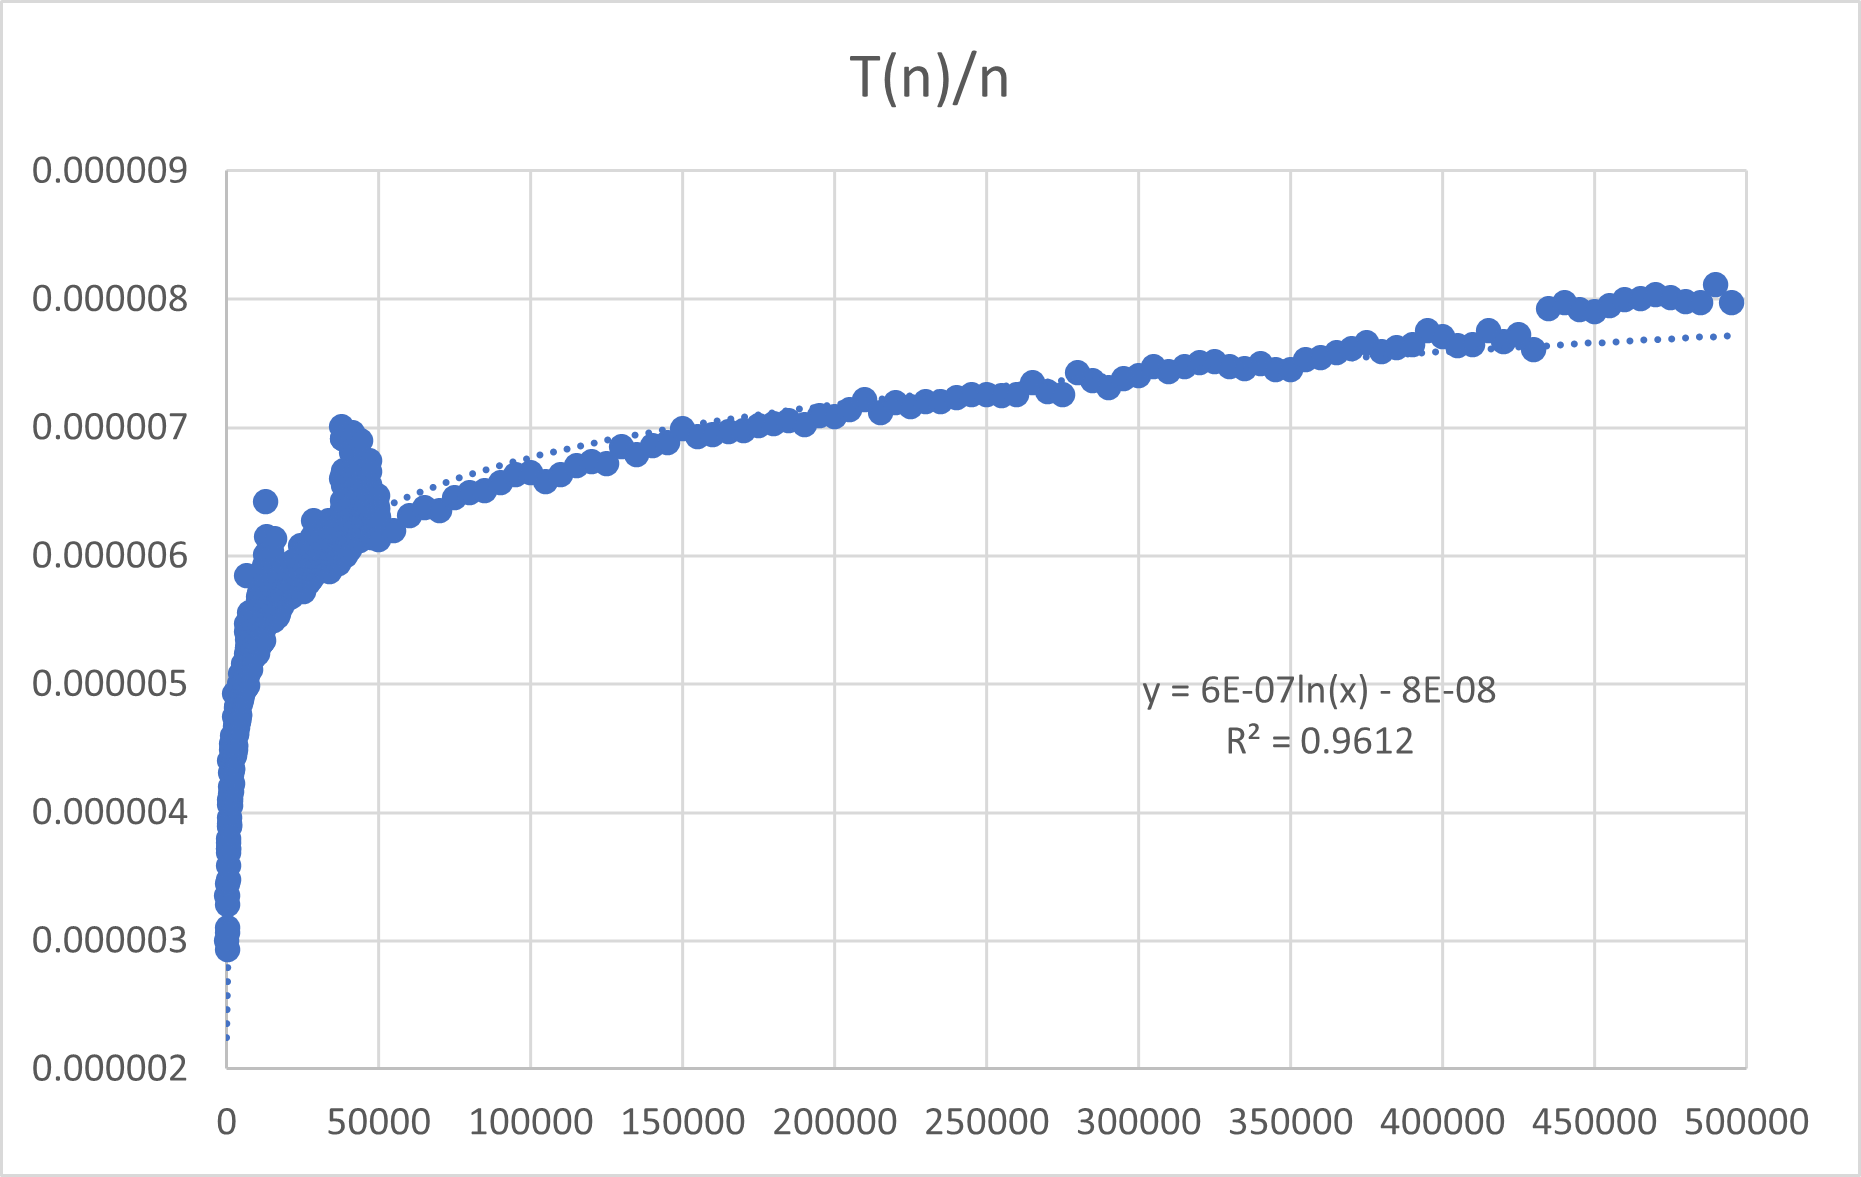
\includegraphics[width=0.6\textwidth,height=\textheight,keepaspectratio]{hn_Tn_n}
\caption{logarithmic fitting for $h(n)$}
\label{Figure: hn_3}
\end{figure}

\noindent The resulting graph appears to be logarithmic. The $R^2$ is 0.9612 for the logarithmic trend line. Therefore we can conclude that $h(n) = O(n\log{n})$.

\section{Python Lists}

\subsection{Copy}
For all three methods in question, very similar testing methods were selected. Since complexity is measured in the "big O" notation, where N is the number of inputs, the overall trend is seen by testing a relatively small number of inputs. 

I decided to start at an array size of 1 and multiply the subsequent array by 10 each time until the array is 1 million in size. Later, I  added additional data points starting at 3 and following similar steps to make my data more complete. 

\footnotesize
\begin{verbatim}
                                  timing for 1 runs
                                  timing for 3 runs
                                  timing for 10 runs
                                  timing for 30 runs
                                  timing for 100 runs
                                  ...
\end{verbatim}
\normalsize
  
The contents of the arrays were different for each method tested. In the case of .copy() the array consisted of random integers between 0 and the size of the array being generated:

\footnotesize
\begin{verbatim}
import random

def arrayGenApp(upperLimit):
  j = 0
  arr = []

  while (j < upperLimit):
    arr.append(random.randint(0,upperLimit))
    j += 1

  return arr
\end{verbatim}
\normalsize

After generating the arrays and measuring the time it took to .copy() each one of them, I received data which I plotted on the graph below. The data was plotted with a log scale to properly show the trend.

The initial flat section is consistent with the similar experiments found online and can be disregarded when analyzing the later data points. (reference)

\begin{figure}[H]
\centering
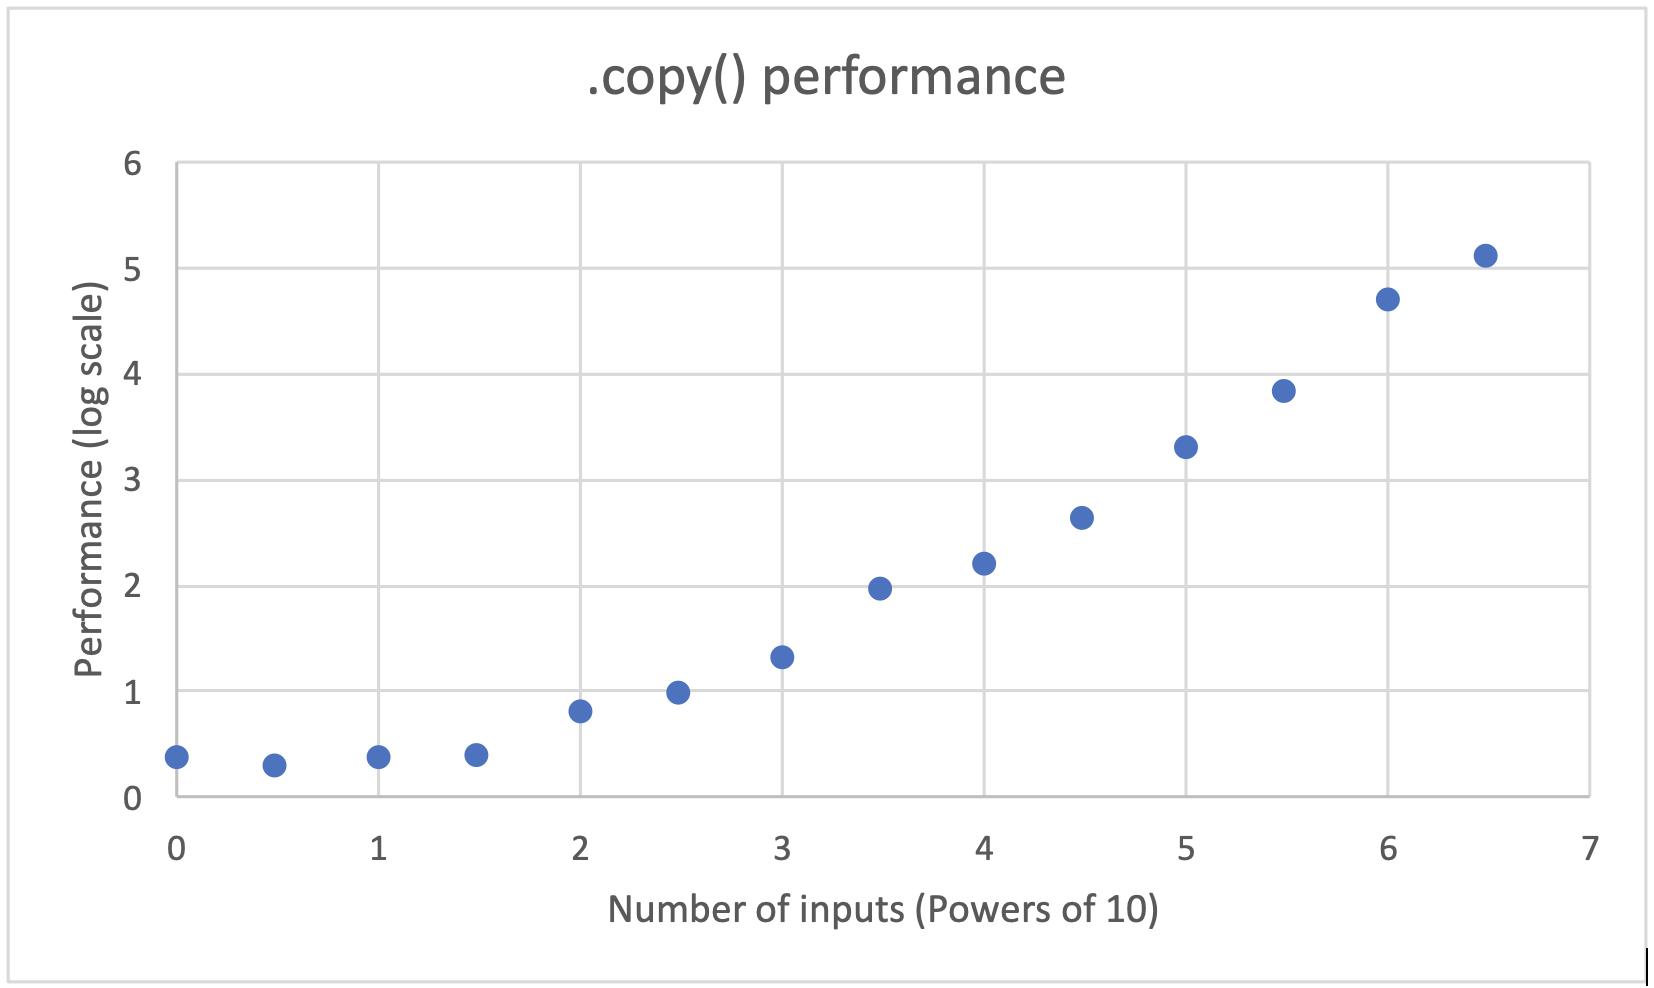
\includegraphics[width=0.6\textwidth,height=\textheight,keepaspectratio]{copygraph.png}
\caption{.copy() performance}
\label{Figure: copygraph}
\end{figure}

Based on official documentation, python's .copy() method runs in O(n) time which is verified by the linear time complexity (justification) seen in the graph. This means that if we double an array size, it would take, on average, double the time to make a copy of it. 

\footnotesize
\begin{verbatim}
def copy(array):

  arrCpy = array.copy()

  return arrCpy
\end{verbatim}
\normalsize

Since array.copy() iterates over each object in an array, adding references to a new array, it is expected that the runtime would be linear.

\subsection{Lookups}

Lookups used a similar testing method to the one described in .copy(). This time, each array consisted of values from 0 to the upper limit in a natural order. For example, an array of size 10 had the values 0,1,2,...8,9. After consulting with the TA's, this was the method I decided to use as it provided a better estimate of lookups for python lists.

\footnotesize
\begin{verbatim}
def arrayGenApp(upperLimit): #values in array increasing
  j = 0
  arr = []
  
  while (j < upperLimit):
      arr.append(j)
      j += 1

  return arr
\end{verbatim}
\normalsize

My prediction for the runtime was that the method would not depend on the size of the array, meaning it would run in constant time O(1). For each lookup the algorithm does not need to traverse the array, instead, it would directly access the element with the given index.

\footnotesize
\begin{verbatim}
def arrayLook(array):
  i = 0
  while (i < len(array)): 
    array[i]
    i += 1
\end{verbatim}
\normalsize

I had a problem with the original formulation of the question because the given instructions would not properly test the lookup method. The correct approach in my opinion was to measure the time it would take to look up each value in different size arrays which is the approach I implemented. 

Not only would this determine if the lookup method is dependent on array size, but also whether it is affected by the length of the variable being accessed. Since with my testing strategy, a larger array would have larger values stored within it.

\begin{figure}[H]
\centering
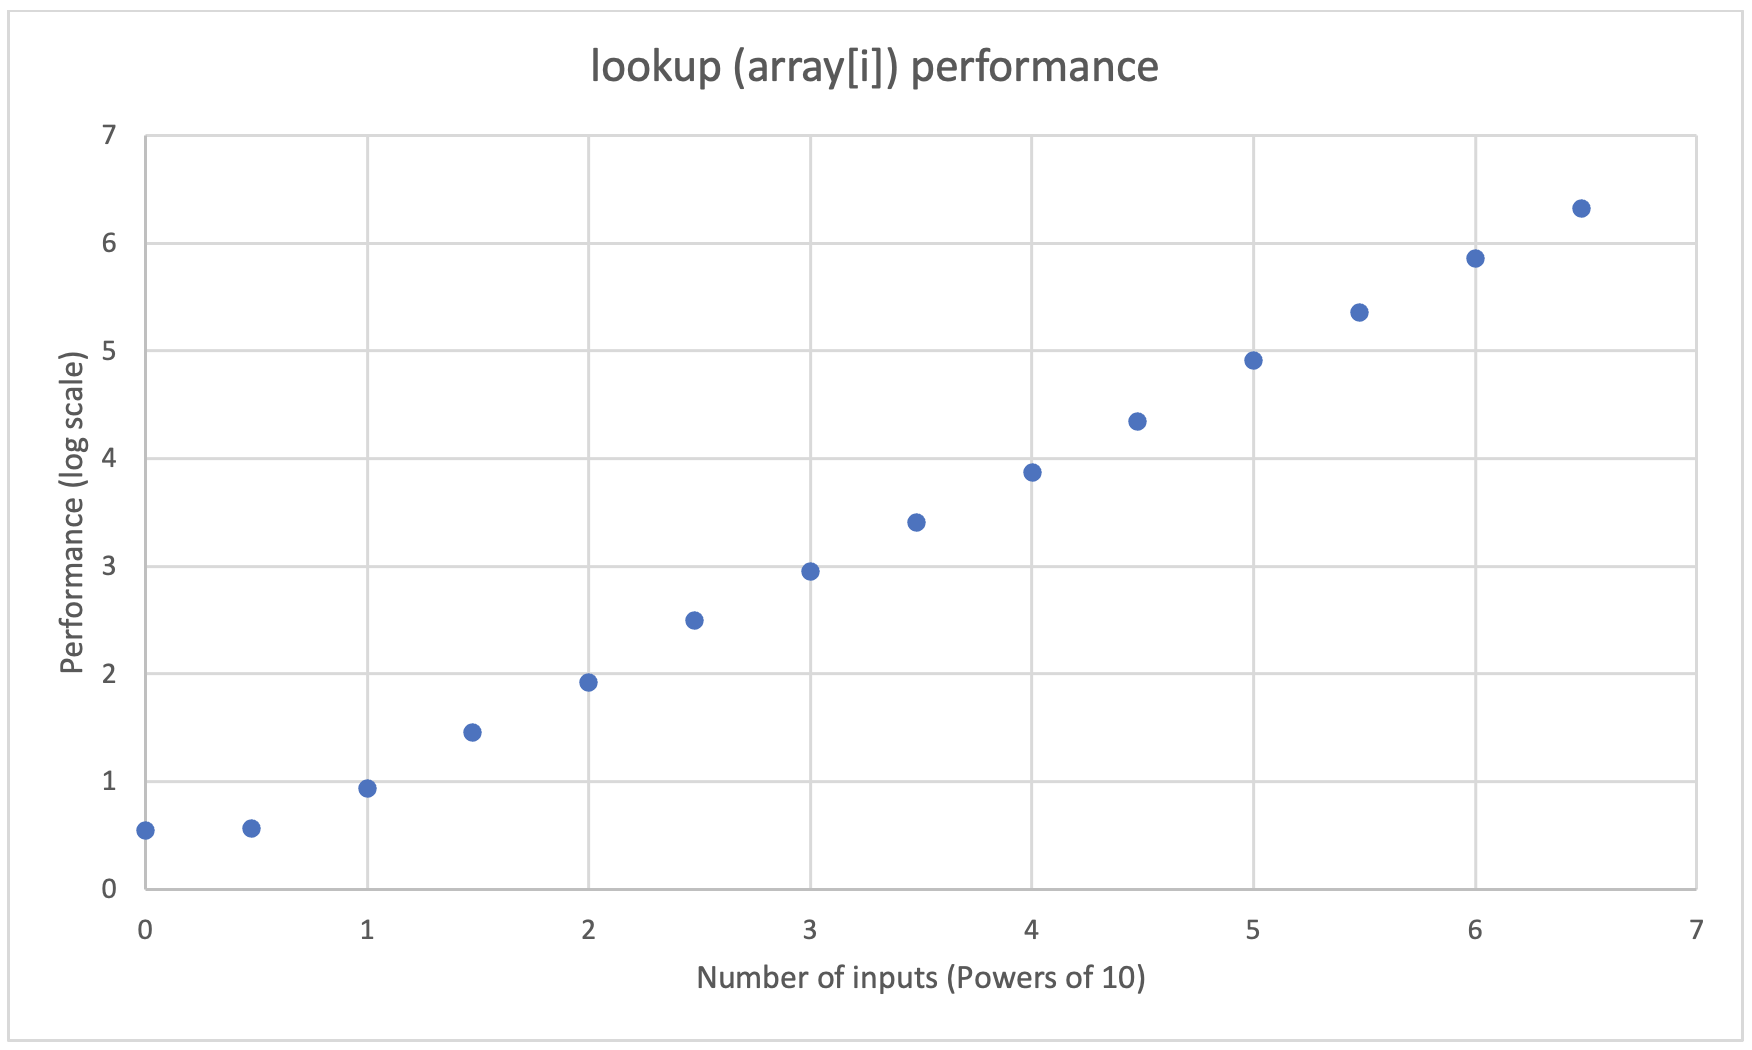
\includegraphics[width=0.6\textwidth,height=\textheight,keepaspectratio]{lookupgraph.png}
\caption{array[i] (lookup) performance}
\label{Figure: lookupgraph}
\end{figure}

\subsection{Append}


\end{document}

